\chapter{Benchmarks and Metrics in Industry}\label{ch:benchmarks_and_metrics}
In this chapter all the tools and the benchmarks for object localization and detection will be exposed. In particular, first the metrics and the techniques used to evaluate pose estimations will be presented, then some publicly available datasets will be presented. 

The problems that are going to be tackled are related to the 6D object pose estimation task. A 6D object pose is mathematically the 3D position of the object in the space plus 3 more terms that describe its rotation:

\begin{equation}
    \label{eq:6D_obj_pose_0}
    \hat{P} = (x, y, z, \alpha_x, \alpha_y, \alpha_z)^T
\end{equation}

The Eq. \ref{eq:6D_obj_pose_0} refers to the 6D pose estimate of an object, the first three terms $x, y, z$ describe the position in the camera reference frame, while the last three terms $\alpha_x, \alpha_y, \alpha_z$ represent the object's rotation angles along the $x, y, z$ camera axis respectively. This formulation can be easily manipulated in terms of rotation matrices and translation vectors:

\begin{equation}
    \label{eq:6D_obj_pose_1}
    \hat{P} = (R, t)
\end{equation}

The Eq. \ref{eq:6D_obj_pose_1} is a manipulated version of \ref{eq:6D_obj_pose_0} where the rotation matrix $R$ encodes the three angles of rotation $\alpha_x, \alpha_y, \alpha_z$ and the translation vector $t$ encodes the $x, y, z$ position of the object in the reference frame of the camera.

\begin{figure}
	\centering
	\begin{subfigure}{.5\textwidth}
  		\centering
  		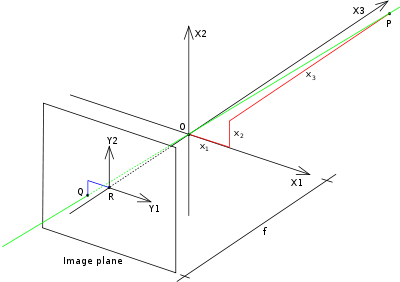
\includegraphics[width=.9\linewidth]{figures/2_benchmarks_and_metrics/pinhole_geometry_3D}
  		\caption{3D view}
  		\label{fig:pinhole_geometry3D}
	\end{subfigure}%
	\begin{subfigure}{.5\textwidth}
  		\centering
  		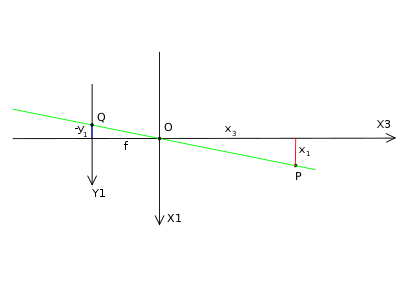
\includegraphics[width=.9\linewidth]{figures/2_benchmarks_and_metrics/pinhole_geometry_2D}
  		\caption{2D view}
  		\label{fig:pinhole_geometry2D}
	\end{subfigure}
	\caption{\textbf{Pinhole Camera Geometry.} In (A) the geometry of the pinhole camera in 3D view, in (B) its 2D representation.}
	\label{fig:pinhole_geometry}
\end{figure}

Each object pose estimate can also be projected back to the camera image plane. This projection between the 3D space and the 2D space of the image plane is achieved by applying the projection obtained with a given camera matrix model. The camera model that we consider here is the so called Pinhole Camera Model, and it's geometry is depicted in Figure \ref{fig:pinhole_geometry}.

The mapping from the coordinates of a 3D point $P$ to the 2D image coordinates of the point's projection onto the image plane, according to the pinhole camera model is given by:

\begin{equation}
    \label{eq:3D_to_2D_mapping}
    x_i = \left[ \begin{array}{c} u \\ v \end{array} \right] = \dfrac{f}{x_3} \left[ \begin{array}{c} x_1 \\ x_2 \end{array} \right]
\end{equation}

In Eq. \ref{eq:3D_to_2D_mapping} $x_1, x_2, x_3$ represent the 3D position in space of a generic point, $f$ is the focal length of the camera, and $u, v$ are the image coordinates obtained after the projection.

The formulation just explained is for an ideal pinhole camera located in the origin and with focal length equal for the $x$ and $y$ axes of the image. Typically, the situation is different, and the more generic formulation is like the following:

\begin{equation}
    \label{eq:generic_pinhole_camera_model}
    x_i = \left[ \begin{array}{c} u \\ v \\ 1 \end{array} \right] = \begin{bmatrix} f_x & 0 & c_x \\ 0 & f_y & c_y \\ 0 & 0 & 1 \end{bmatrix} \left[ \begin{array}{c} x_1 \\ x_2 \\ x_3 \end{array} \right]
\end{equation}

In Eq. \ref{eq:generic_pinhole_camera_model} the camera is formulated using its internal parameter $f_x, f_y, c_x, c_y$ that represent respectively the two focal lengths on the $x, y$ image axis and the camera optical center $(c_x, c_y)^T$.

With Eq. \ref{eq:3D_to_2D_mapping} and \ref{eq:generic_pinhole_camera_model} we can project each point of the 3D object model onto the image plane and compare the estimated pose with the ground truth one following one of the metrics that are going to be explained in the sections below.

\section{Metrics}\label{sec:metrics}
The problem of evaluating how good is a pose estimate w.r.t. the ground truth is a challenging and still very open topic in computer vision community.  Taking inspiration from \cite{hodan20166DPoseEstimation} we will first focus on bounding box estimates comparison and then will pass to the more complex and challenging problem of compare two object 6D pose estimate.

\begin{figure}
    \centering
    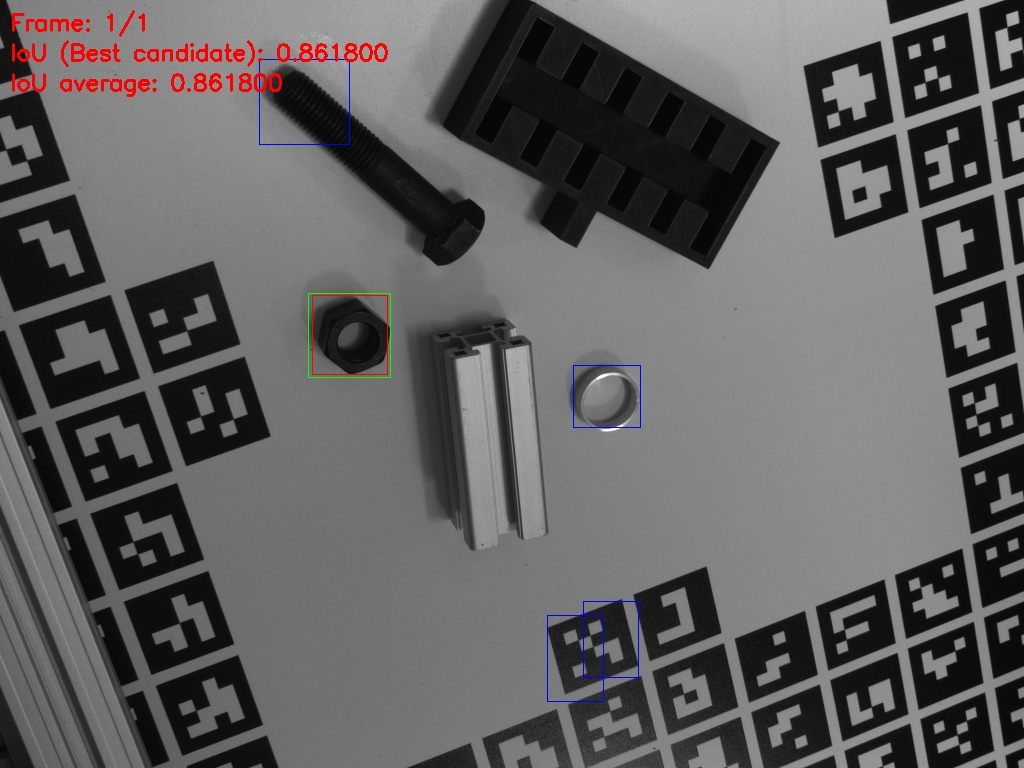
\includegraphics[width=0.7\textwidth]{figures/2_benchmarks_and_metrics/iou_example}
    \caption{\textbf{IoU score estimation example.} An eample of estimating the 2D bounding box of an object, in particular, the small nut, called M20 in the RAW dataset, with the Halcon Libraries. In red the ground truth bouning box, in green the Halcon best candidates, in blue the last two best candidates.} 
    \label{fig:iou_example}
\end{figure}

\subsection{2D Intersection over Union (IoU)}\label{subsec:iou}
The most common way to measure accuracy of object detection in 2D domain is to calculate the Intersection over Union score \cite{everingham2015challenge}:

\begin{equation}
    \label{eq:iou_score}
    s_{IOU}(\hat{B}, \bar{B}) = \dfrac{area(\hat{B} \cap \bar{B})}{area(\hat{B} \cup \bar{B})}
\end{equation}

In Eq. \ref{eq:iou_score} $\hat{B}$ and $\bar{B}$ are the estimated and ground truth 2D region respectively. Depending on the task, $\hat{B}$ and $\bar{B}$ can be rectangular regions (given by bounding boxes) or segmentation masks. For evaluation of 6D object pose estimates, the 2D regions can be obtained by projection of the object model $\mathit{M}$ in the estimated pose $\hat{P}$ and the ground truth pose $\bar{P}$ . Such pose error function is ambiguity-invariant, but since it operates in the projective space, it provides only a weak information about fitness of the object surface alignment. That basically means that every projection of the model that realizes in the same bounding box will have the very same score, even if the object is completely flipped among the two 6D poses. It is said that the IoU score is not ambiguity-invariant, we will see in the further section what ambiguity is. 

That is the reason why we only consider IoU for 2D measurement comparison, and so, only for object detection tasks, where just the location of the object within the image plane is considered to be interesting, not its exact position and orientation in 3D space. Examples of bounding boxes comparison, so IoU estimation is given in Figure \ref{fig:iou_example}. Usually a object detection is considered correct, when the IoU score of 2D bounding boxes of an object in the estimated and the ground truth pose is above a
threshold (e.g. 0.5).

\subsection{5cm, 5deg Criteria}\label{subsec:5cm5deg}
After having introduced the metrics used for comparing object detection estimates, we now pass to tackle the problem of estimating the ``goodness'' of a 6D pose estimate. In the introduction of chapter \ref{ch:benchmarks_and_metrics} we formulated the pose of an object in 3D space in terms of rotation  matrix and translation vector, as stated in Eq. \ref{eq:6D_obj_pose_1}. From this simple formulation, intuitively, a simple error function can be built, in particular we can consider the error of the estimated pose $\hat{P} = (\hat{R}, \hat{t})$ w.r.t. the ground truth pose $\bar{P} = (\bar{R}, \bar{t})$ as composed by two independent terms, the translational error $(e_{TE})$ and the rotational error $e_{RE}$ respectively. These errors can be used as a metric for the computation of the goodness of a 6D pose estimate.

More in detail, the aforementioned $e_{TE}$ and $e_{RE}$ can be mathematically expressed as:

\begin{equation}
    \label{eq:translational_error}
    e_{TE}(\hat{t}, \bar{t}) = \norm{\hat{t} - \bar{t}}_2
\end{equation}

\begin{equation}
    \label{eq:rotational_error}
    e_{RE}(\hat{R}, \bar{R}) = arccos(\dfrac{Tr(\hat{R}\bar{R}^{-1}) - 1}{2})
\end{equation}

In particular, Eq. \ref{eq:translational_error} is simply the squared distance from the 2 points represented by their respective translation vectors $\hat{t}$ and $\bar{t}$, and Eq. \ref{eq:rotational_error} represents the rotational error in the axis-angle representation of the rotation matrices $\hat{R}$ and $\bar{R}$. More over, in $e_{RE}$, the function $Tr()$ is the trace of the rotation matrix.

After the previous formulation, we can now introduce a simple and intuitive criteria for evaluating the goodness of a 6D pose estimate. In \cite{shotton2013coordinate}, the so called \emph{5cm, 5deg} criteria have been introduced. It simply states that it is considered a good pose estimate if and only if $e_{TE} \leq 5cm$ and $e_{RE} \leq 5deg$. Of course, more general formulation of the same criteria can be used, by imposing variable thresholds $t_{TE}$ and $t_{RE}$ in the place of the constants $5cm$ and $5deg$.

This criteria was initially used for evaluating camera pose estimations, and it perfectly fits the case, but in terms of computing the goodness of a 6D object pose estimate, it is not adaptive to object model projections, in the sense that 2 different poses that refer to 2 different model projection onto the image plane can assume the very same $e_{TE}$ and $e_{RE}$, so those errors are still not ambiguity-invariant, as like as the IoU score.

\subsection{Pose Ambiguity Invariant Metrics}\label{subsec:pose_ambig_invariant_metrics}
Before introducing the idea of Average Distance for model points let's introduce the concept of \emph{Indistinguishable Poses} and \emph{Invariance to Pose Ambiguity}. As anticipated in the last two sections, IoU score and rotational and translational errors are not invariant to pose ambiguities, so let's see what this concern before introducing how we can overcome this issue.

\subsubsection{Indistinguishable Poses}\label{subsubsec:indistinguishable_poses}
If we take as example a generic object model, call it $M$, we can define a class of \emph{indistinguishable} poses for this model with the following:

\begin{equation}
    \label{eq:indistinguishable_poses}
    [P]_{M,I,\epsilon} = {P^{\prime} : d(v_I[PM], v_I[P^{\prime}M]) \leq \epsilon}
\end{equation}

where $v_I[M] \subseteq M$ is that part of the object model M that is actually visible in the image $I$, that is not self-occluded or occluded by some other object, $d$ is a distance between the surfaces, and $\epsilon$ is a threshold that basically controls the level of detail that we want to achieve in comparing two different views of the same model in the image.

\subsubsection{Invariance to Pose Ambiguity}\label{subsubsec:pose_ambiguity_invariance}
Pose Ambiguity is a necessary property for a 6D object pose estimator. Given an image $I$, a model $M$ and an estimated pose $\hat{P}$, the error $e(\hat{P}, \bar{P}; M, I)$ is required to be invariant under pose ambiguity iff:

\begin{equation}
    \label{eq:pose_ambiguity_invariance}
    \forall \hat{P}^\prime \in [\hat{P}]_{M, I, \epsilon},
    \forall \bar{P}^\prime \in [\bar{P}]_{M, I, \epsilon} : 
    e(\hat{P}^\prime, \bar{P}^\prime) \approx e(\hat{P}, \bar{P})
\end{equation}

where the approximation is given because of the $\epsilon$ tolerance term. A pose error function $e$ that satisfy such property is called \emph{ambiguity-invariant}.

This property is extremely important because an 6D object pose estimator relies its estimates only on the single image, there is no tracking information, and any other spatial relation with the model pose in the image that can distinguish two different pose estimates, so pose ambiguity cannot be removed in any way, that is why we need to model it somehow.

\subsubsection{Average Distance (AD)}\label{subsubsec:average_distance}
When the sets of visible points for the model $M$ in the image $I$ is available, one possible solution to estimate how good is the detected pose $\hat{P}$ is to evaluate the average of the maximum of distances between corresponding points of model $M$ for each pose pair $(\hat{P}, \bar{P}) \in Q = [\hat{P}]_{M, I, \epsilon} \times [\bar{P}]_{M, I, \epsilon}$, and finally take the minimum of those average distances:

\begin{equation}
    \label{eq:average_distance}
    d_h((\hat{R}, \hat{t}), (\bar{R}, \bar{t}); M) = \dfrac{1}{|M|}  \sum\nolimits_{x_1 \in M} \min_{x_2 \in M} \norm{(\hat{R}x_1 + \hat{t}) - (\bar{R}x_2 + \bar{t})}_2
\end{equation}

This distance is very intuitive, but not so effective, and we will see whit an example in the following subsection why take the maximum instead of the average, is a more convenient way.

\begin{figure}
    \centering
    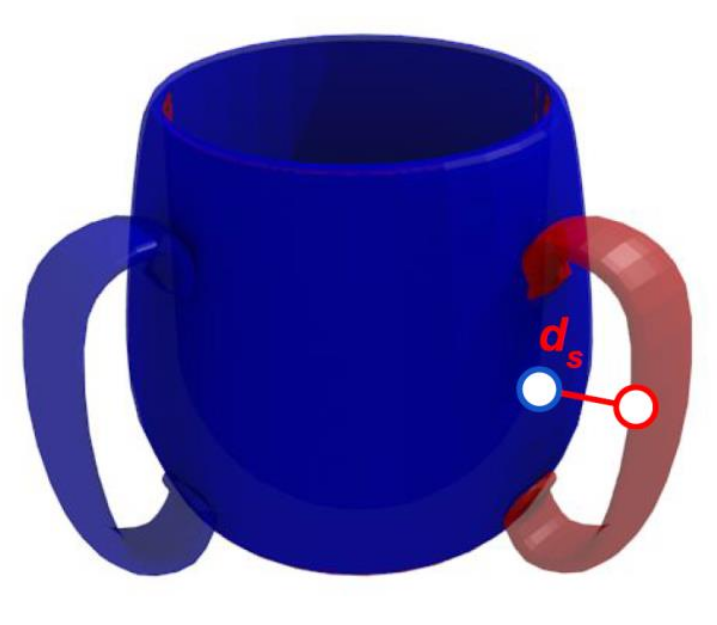
\includegraphics[width=0.5\textwidth]{figures/2_benchmarks_and_metrics/max_av_distances_example}
    \caption{\textbf{Maximum vs Average Distance.} In this example, it is perfectly shown how taking the maximum instead of the average, is much more convenient. For the mug depicted in the picture, the blue pose (the ground truth), and the red one (the estimation) have very low average distance, while high maximum distance. This explain how maximum distance is more convenient for this case, it reflects better the misalignment between the two poses. The average distance $d_h$ cannot be drawn here, because this distance does not relates with any geometrical points, it's just a score.} 
    \label{fig:max_av_distances_example}
\end{figure}

\subsubsection{Maximum Distance (MD)}\label{subsubsec:maximum_distance}
As anticipated in the last section, taking the maximum instead of the average, can be more effective, also compared with the task that we want to perform. Imagine to take a mug, like in the example in Figure \ref{fig:max_av_distances_example}, where the Maximum Distance $d_s$ is calculated performing the maximum instead of the average:

\begin{equation}
    \label{eq:maximum_distance}
    d_s((\hat{R}, \hat{t}), (\bar{R}, \bar{t}); M) = \max_{x_1 \in M} \min_{x_2 \in M} \norm{(\hat{R}x_1 + \hat{t}) - (\bar{R}x_2 + \bar{t})}_2
\end{equation}

Whit this little modification to the formulation of the distances, the situation completely changes. In the example in Figure \ref{fig:max_av_distances_example} the distance $d_s$ reflects better the misalignment between the estimated pose and the ground truth. But, is this the right choice? Is this distance reflecting all the necessary when estimating the pose of the mug? In Figure \ref{fig:ds_vs_dp} there is another possible distance that can reflect better the misalignment between ground truth and estimated pose. It is clearly evident that maybe the new distance $d_p$, is better that the maximum distance $d_s$. So we need to find a solution to this problem, and one possible way is to introduce the concept of \emph{equivalence classes}, and then calculate the distances also considering them.

Considers all poses from the equivalence class $[(\hat{R}, \hat{t})]$ of the ground truth pose (given by pre-defined symmetries of the object), we can define the new distance $d_p$ with the following:

\begin{equation}
    \label{eq:maximum_distance_eq_classes}
    d_p((\hat{R}, \hat{t}), (\bar{R}, \bar{t}); M) = \min_{(\hat{R}, \hat{t}) \in [(\hat{R}, \hat{t})]} \max_{x \in M} \norm{(\hat{R}x + \hat{t}) - (\bar{R}x + \bar{t})}_2
\end{equation}

This new distance reflects better the misalignment between ground truth pose and estimated one, facilitating the evaluation of the pose estimate in tasks like robot grasping and others.

\begin{figure}
    \centering
    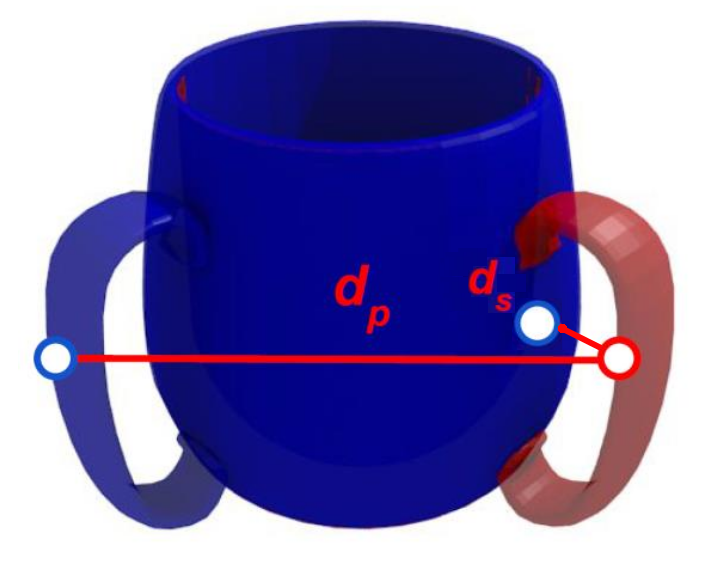
\includegraphics[width=0.5\textwidth]{figures/2_benchmarks_and_metrics/ds_vs_dp}
    \caption{\textbf{Maximum Distance ambiguities.} In this example it is clearly evident that the distance $d_p$ better reflects the misalignment w.r.t. the $d_s$ one.} 
    \label{fig:ds_vs_dp}
\end{figure}

\subsubsection{Visible Surface Distance (VSD)}\label{subsubsec:visible_surface_distance}
Do we need actually to perform the evaluation of the distance $d_p$ for all the points of the model $M$. It is actually a very computationally expensive task. That is why we now introduce the concept of \emph{Visible Surface}. The key-point here is to evaluate the distance only on the visible part of the model within the image:

\begin{equation}
    \label{eq:vis_surf_error}
    e_{VSD}(\hat{P}, \bar{P}; M, I, \delta, \tau) = avg_{p \in \hat{V} \cup \bar{V}} c(p, \hat{D}, \bar{D}, \tau)
\end{equation}

In Eq. \ref{eq:vis_surf_error}, $\hat{V}$ and $\bar{V}$ are the 2D masks of the visible surface of the projected models, with the ground truth pose $\hat{P}$ and the estimated pose $\bar{P}$ respectively. $\hat{D}$ and $\bar{D}$ are the \emph{distance images} obtained by rendering the two models in the camera reference frame. $\delta$ is a tolerance threshold used for the computation of the visibility masks, and $c(p, \hat{D}, \bar{D}, \tau) \in [0, 1]$ is the matching cost at pixel $p$:

\begin{equation}
    \label{eq:matching_cost_at_p}
    c(p, \hat{D}, \bar{D}, \tau) = \left\{
\begin{array}{c l}	
     \dfrac{d}{\tau} & if p \in \hat{V} \cap \bar{V} \wedge d > \tau \\
     1 & otherwise,
\end{array}\right.
\end{equation}

More in detail, in Eq. \ref{eq:matching_cost_at_p}, the distance image $d$ is given by:

\begin{equation}
    \label{eq:distance_image}
    d = |\hat{D}(p) - \bar{D}(p)|
\end{equation}

and it can be easily derived from the two depth images of the ground truth and the estimated poses respectively

In order to better understand the concept of visible surface, and the role of the visibility masks $\hat{V}$ and $\bar{V}$ in the equations \ref{eq:vis_surf_error} and \ref{eq:matching_cost_at_p}, let's take as example the mug depicted in Figure \ref{fig:visibility_mask_ex}.

\begin{figure}
    \centering
    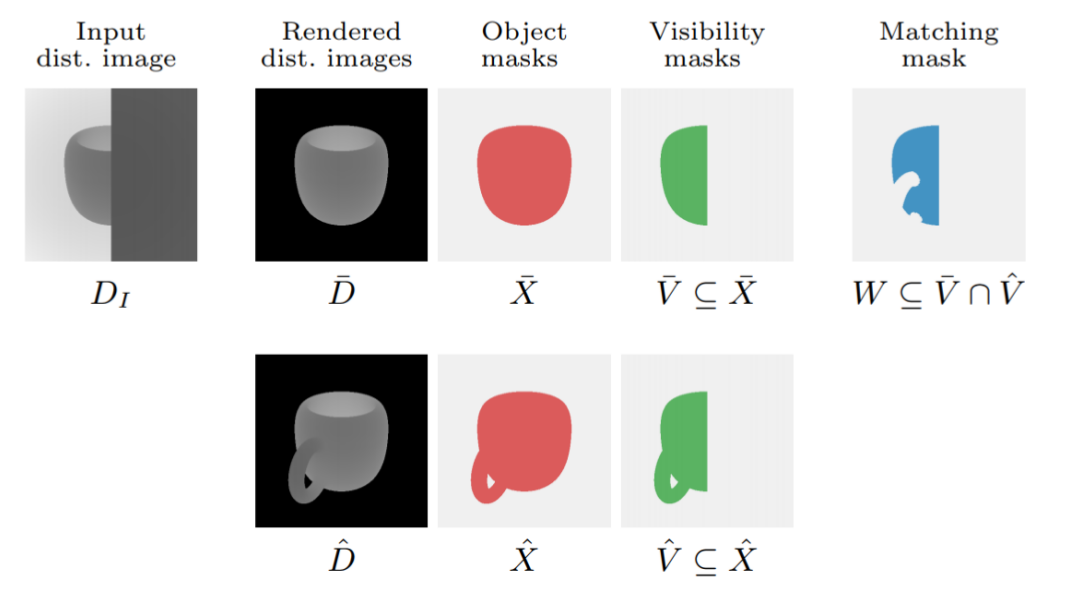
\includegraphics[width=0.8\textwidth]{figures/2_benchmarks_and_metrics/visibility_mask_ex}
    \caption{\textbf{Visibility Masks Example.} An example of how to compute the visibility mask for the mug in the image.}
    \label{fig:visibility_mask_ex}
\end{figure}

\section{Industrially Oriented Datasets}\label{sec:datasets}
After having introduced and formulated the metrics used for comparing object detection and pose estimation measurements, we can now introduce some benchmark tools and data used for industrial applications. Typical settings are those with \emph{texture-less} objects, namely, objects that do not present any kind of texture. Given this property, object detectors and pose estimators can rely their estimations only on shape based approaches, without any sort of rbg texture based techniques.

Examples of texture-less datasets are the \emph{T-LESS} Dataset \cite{hodan2017tless} from the Center for Machine Perception of the Czech Technical University of Prague and the \emph{MVTec ITODD Dataset} \cite{mvtec2017itodd} from the same company that distributes the Halcon Libraries.

\begin{figure}
    \centering
    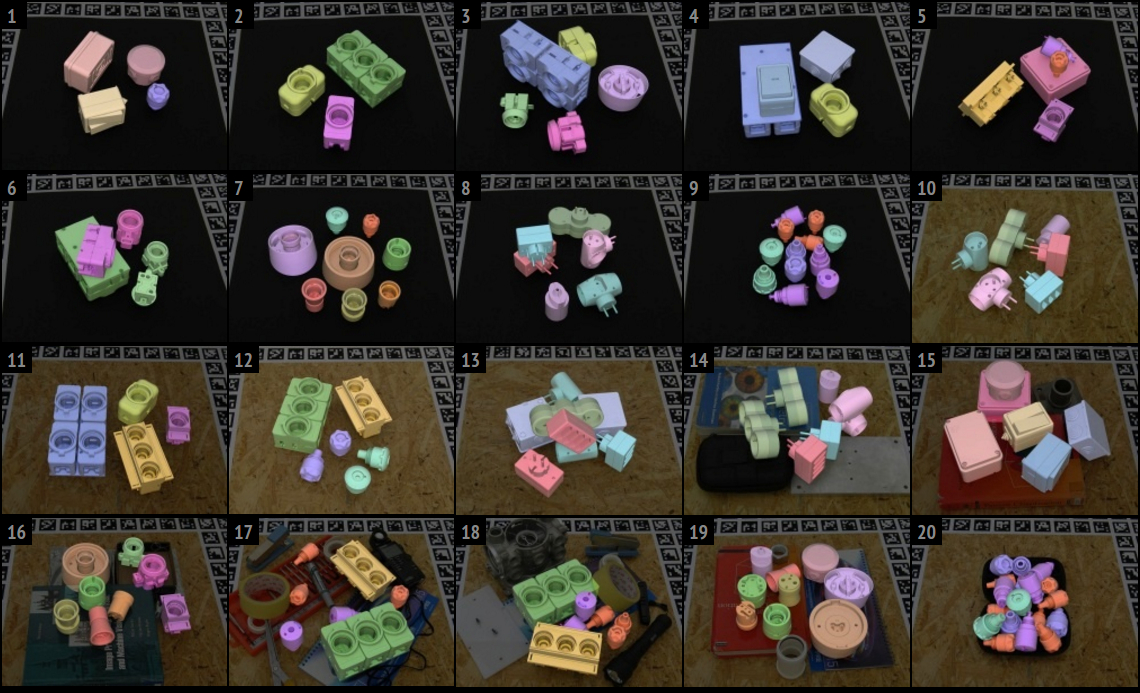
\includegraphics[width=0.8\textwidth]{figures/2_benchmarks_and_metrics/tless_ex_scenes}
    \caption{\textbf{T-LESS scenes examples.} A compact view of the scenes present in the T-LESS dataset.}
    \label{fig:tless_ex_scene}
\end{figure}

\subsection{T-LESS Dataset}\label{subsec:tless_dataset}
The T-LESS Dataset \cite{hodan2017tless}, has the name suggests, is a publicly available dataset\footnote{http://cmp.felk.cvut.cz/t-less/index.html} composed by thirty different texture-less objects. All the objects in the dataset are from the industrial scenario and do not present any particular feature, moreover, most of them are also very similar in shape and color.

The dataset is composed by training and test images, the former are represented by RGB and RGB-D images of multiple views of the single object, while the latter are composed by 21 test scenes where the objects are collected together in more cluttered and unstructurated forms. All the scenes, both training and test ones, have been acquired with a fixed sensor setup composed by the following RGB and RGB-D cameras:

\begin{itemize}
	\item Primesense Carmine 1.09 (Short Range) that provides registered RGB-D images with the following features: RGB:1280x1024 px, Depth:640x480 pixels;
	\item Microsoft Kinect v2 that provides images with registered depth with 1920x1080 pixels of resolution;
	\item Canon IXUS 950 IS high resolution camera that provides RGB images of 3264x2448 pixels of resolution.
\end{itemize}

All the three sensors have been mounted on a fixed structure and a rotating turntable with the objects on top has been built for positioning and rotating the training and test scenes. Examples of acquired scenes are in Figure \ref{fig:tless_ex_scene}.

In the T-LESS data packages also the CAD models of the objects are given to the public. In particular they released two different kind of CAD models:

\begin{itemize}
	\item Manually created CAD models;
	\item Automatically reconstructed CAD models.
\end{itemize}

%\begin{figure}
%    \centering
%    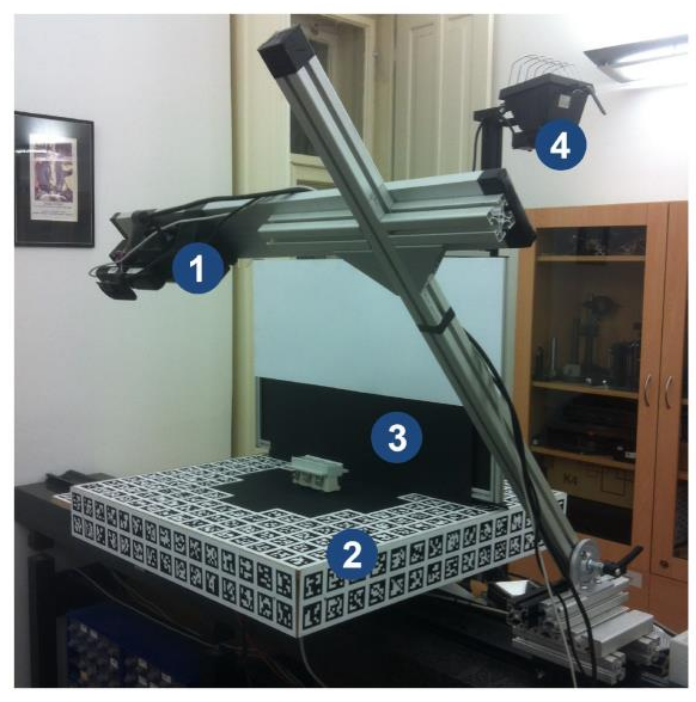
\includegraphics[width=0.9\textwidth]{figures/%2_benchmarks_and_metrics/tless_sensor_setup}
%    \caption{\textbf{T-LESS sensor setup.} The setup of the %sensors used during the acquisition of the T-LESS scenes. In the %picture}
%    \label{fig:tless_sensor_setup}
%\end{figure}

\begin{figure}
    \centering
    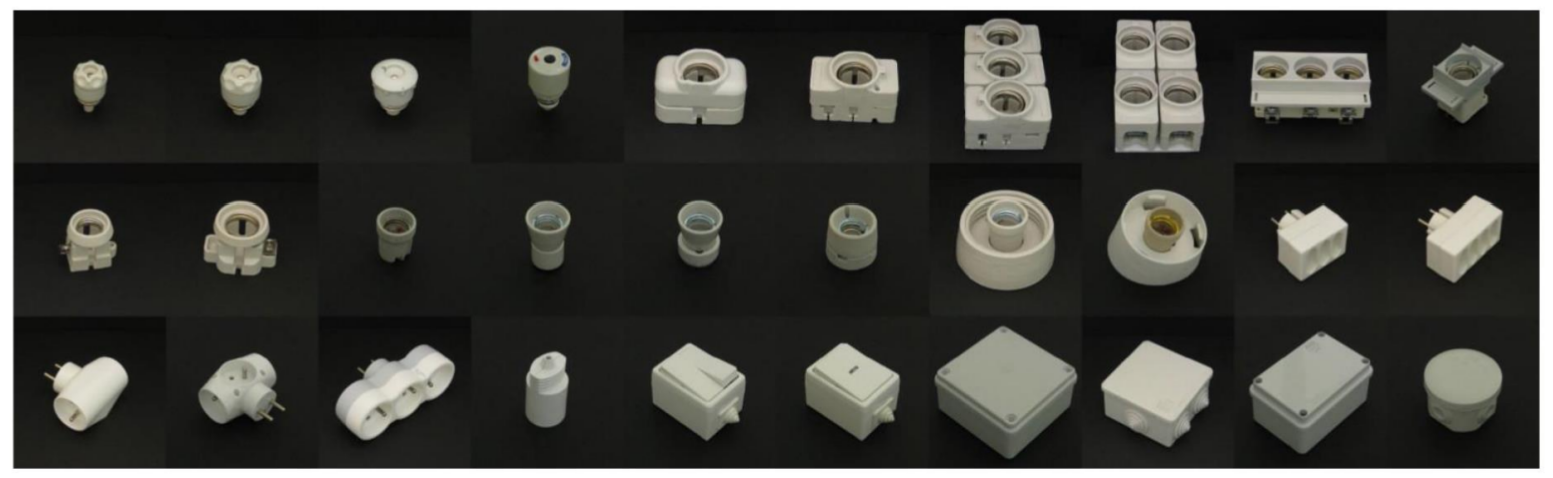
\includegraphics[width=0.9\textwidth]{figures/2_benchmarks_and_metrics/tless_objs_ex}
    \caption{\textbf{T-LESS Objects Samples.} A compact view of the thirty object classes present in the T-LESS dataset.}
    \label{fig:tless_objs_ex}
\end{figure}

All the objects presented in the T-LESS dataset are also shown here in Figure \ref{fig:tless_objs_ex}. As like as for our RAW dataset, they organized their objects in multiple scenes, 21 as already mentioned, classified by order of complexity: \emph{easy} and \emph{hard} objects scenes. Each scene has been accurately annotated, and all the objects in it have been localized following the approach explained below:

\begin{enumerate}
	\item A dense 3D model of the scene was reconstructed with the system from \cite{steinbrucker2014volumetric}. This was accomplished using all 504 RGB-D images of the scene along with the sensor poses estimated using the turntable markers;
	\item The CAD models were then manually aligned to the scene model;
	\item To increase accuracy, high-resolution images from Canon camera sensor were used to refine manually all the detected misalignments;
	\item The final poses were distributed to all the test images with the aid of the known camera-to-turntable coordinate transformations.
\end{enumerate}

\begin{figure}
    \centering
    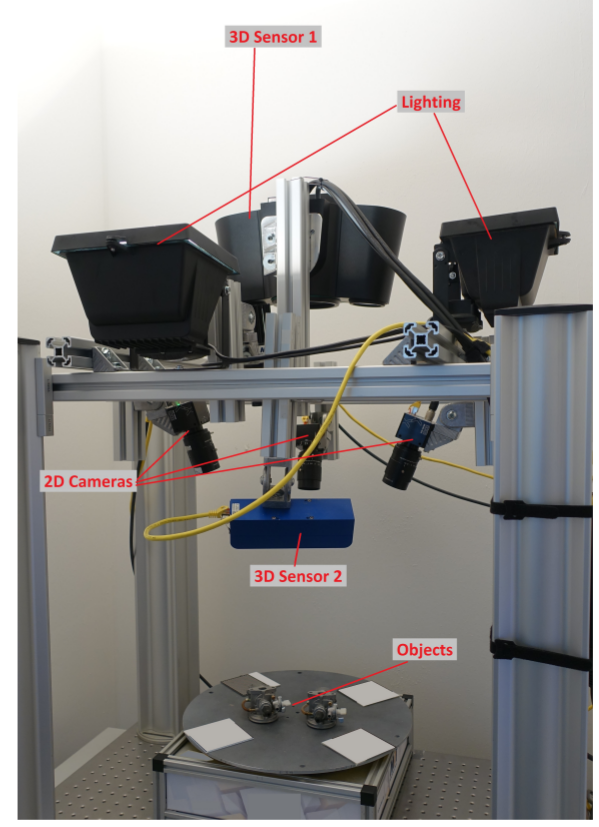
\includegraphics[height=0.4\textheight]{figures/2_benchmarks_and_metrics/itodd_sensor_setup}
    \caption{\textbf{MVTec ITODD Sensor Setup.} In the picture there is a compact view of the fixed sensor setup used for the acquisition of the MVTec ITODD dataset scenes.}
    \label{fig:itodd_sensor_setup}
\end{figure}

\subsection{MVTec ITODD}\label{subsec:mvtex_itodd}
MVTec Industrial 3D Object Detection Dataset, MVTec ITODD \cite{hodan20166DPoseEstimation} in code, is a public dataset for 3D object detection and pose estimation also related to industrial setups, like the previously mentioned T-LESS dataset. The dataset contains 28 object classes, disposed in 800 different scenes, all labeled with 3D rigid transformations with respect to the camera sensors.

The sensors used during the acquisition of the scenes are composed as follow:

\begin{itemize}
	\item High-Quality 3D sensor: a multi-shot 3D stereo sensor that provided both a depth image and a grayscale image with the same viewpoint of the previous one. This sensor also provided high-quality 3D reconstructed cloud of the scene by using multiple random projected patterns and a spacetime stereo approach for reconstructing the scene with an accuracy of around 100 $\mu m$;
	\item Low-Quality 3D sensor: very similar to the previous sensor but with a shorter baseline, a wider field of view and less shots per scene. Given those features, the 3D reconstructed scene is much more noisy than the previous one, with an accuracy of around 1-2 mm;
	\item 3 High.Resolution Cameras: they provided grayscale images, and the scenes where captured twice, one time with the random patterns and the last time without. 
\end{itemize}

In Figure \ref{fig:itodd_sensor_setup} there is a compact view of the fixed sensor setup used for the acquisition of the scenes in the dataset.

\begin{figure}
    \centering
    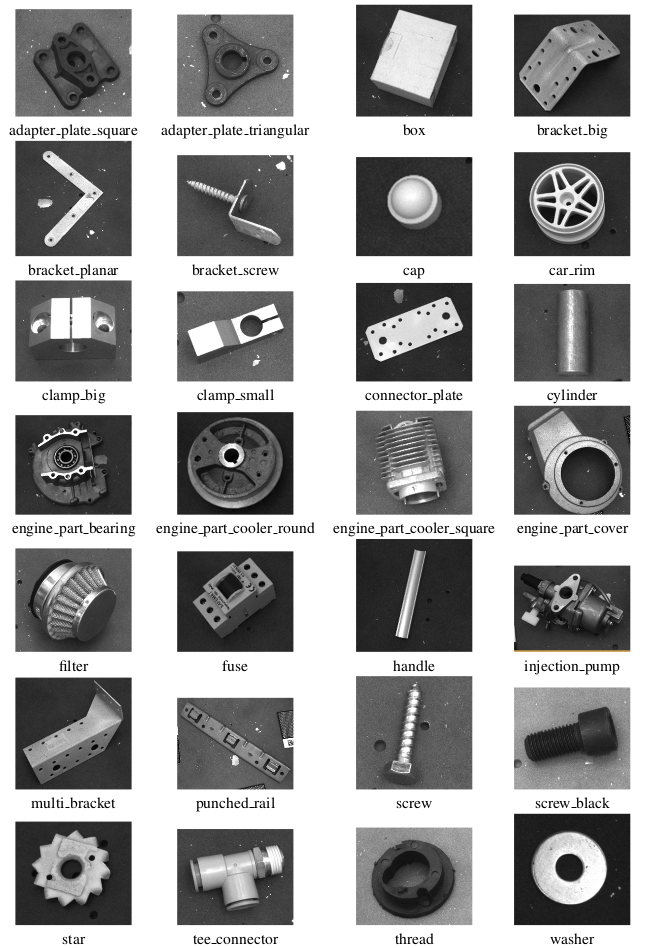
\includegraphics[width=0.8\textwidth]{figures/2_benchmarks_and_metrics/itodd_object_examples}
    \caption{\textbf{MVTec ITODD Object Classes.} All the 28 object classes of texture-less object used during the acquisition of the MVTec ITODD dataset scenes.}
    \label{fig:itodd_object_examples}
\end{figure}

As like as for the T-LESS dataset and the RAW Dataset that we are going to present in the next chapter, the object in the MVTec ITODD dataset are texture-less objects, that is for remarking again the high orientation to the industrial settings of these kind of works. All the object classes used in the MVTec ITODD dataset are depicted in Figure \ref{fig:itodd_object_examples}.

The ground truth 3D pose of all the objects in the MVTec ITODD scenes have been annotated using a T-LESS similar approach. It consists in a semi-manual procedure based on 3D reconstruction and ICP alignment. Once the pose in the first view of the scene has been labeled, this pose has been propagated to all the other view of the scenes by means of the rotating turntable with markers on top.